% L13a student companion deck: synthetic markets with jump hidden Markov models.
% A review of Wolfram markets (placeholder panels), the Two Sigma company profile, a short
% section on Markov chains and hidden Markov models (the full version is the advanced Markov
% notebook), the jump hidden Markov model of one asset, and the sector factor model of many
% stocks. Restructured November 13, 2026, to mirror the restructured lecture.
% Same day: the Markov section mirrors the lecture's theorem-style boxes: a Markov chain
% definition, a proposition for the maximum likelihood estimate of P (its own frame),
% and a hidden Markov model definition.
% Same day: a "Review: Factor Models" frame (the general factor model and the single index
% model's uncorrelated residuals) opens the Many Assets section, as in the lecture.
%
% November 3, 2026. The frame order mirrors the lecture notebook. The disclaimer is
% slide 2, by instructor preference. Notation follows the lecture: state space
% \mathcal{S}, transition matrix \mathbf{P} with entries p_{ij}, estimate \hat{p}_{ij},
% stationary distribution \bar{\pi}, daily growth rate g_t
% (1/yr), jump probability \epsilon and mean episode length \lambda, and the sector
% factor model g_i = alpha_i + beta_i g_m + delta_i f_s + psi_i eps_i.
\documentclass[aspectratio=169,11pt]{beamer}
\usepackage{vnslides}

\newcommand{\Sc}{\mathcal{S}}
\newcommand{\Pb}{\mathbf{P}}
\newcommand{\repo}{https://github.com/varnerlab/CHEME-5660-CourseRepository-Fall-2026/blob/main/lectures/week-13/L13a}

\title{\texorpdfstring{{\vnheavy L13a}}{L13a}: Synthetic Markets with Jump Hidden Markov Models}
\subtitle{CHEME 5660 Cornell University}
\author{Copyright Jeffrey Varner 2026. All Rights Reserved}

\begin{document}

\vntitlepage

\begin{frame}{Disclaimer and Risks}
  \vspace{0.6em}
  \textbf{\ink{Training only.}} This content is for training and informational
  purposes only. The teaching team does not make, give, or endorse any offer or
  solicitation to buy or sell securities or derivative products, or provide
  investment or trading advice or strategy.

  \vspace{1.1em}
  \textbf{\ink{Risk.}} Trading involves risk and is generally not recommended for
  those with limited resources, experience, or a low risk tolerance. Past
  performance does not guarantee future success.

  \vspace{1.1em}
  \textbf{\ink{Responsibility.}} You are responsible for your investment decisions
  based on your financial circumstances, objectives, risk tolerance, and
  liquidity needs.
\end{frame}

\begin{frame}{Objectives for Today}
  Today, we build synthetic markets: simulated price histories with the features of
  real ones. How would a trading method do on thousands of plausible paths?

  \vspace{0.5em}
  {\large\textbf{\ink{Today's concepts}}}
  \begin{itemize}\setlength{\itemsep}{0.4em}
    \item \hilite{Markov chains and hidden Markov models}: states, transition
      matrices, stationary distributions, emissions.
    \item \hilite{A jump hidden Markov model of one asset}: binned states, counted
      transitions, Student-t emissions, jump episodes.
    \item \hilite{A synthetic market of many stocks}: shared market and sector draws
      plus each stock's own draw.
  \end{itemize}
\end{frame}

\begin{frame}{What You Need to Know}
  \vspace{0.3em}
  {\large\textbf{\ink{Core concepts}}}
  \begin{itemize}\setlength{\itemsep}{0.4em}
    \item A Markov chain is a set of states $\Sc$ and a transition matrix $\Pb$ whose
      rows sum to one; its stationary distribution satisfies $\bar{\pi}=\bar{\pi}\Pb$.
    \item The jump hidden Markov model bins the daily growth rate into states,
      estimates $\Pb$ by counting, and draws each day from a Student-t of the day's
      state. Jump episodes (probability $\epsilon$, mean length $\lambda$) keep
      volatility clustering.
    \item A synthetic stock is
      $g_{i}=\alpha_{i}+\beta_{i}\,g_{m}+\delta_{i}\,f_{s}+\psi_{i}\,\tilde{\varepsilon}_{i}$:
      shared market and sector draws make stocks move together.
  \end{itemize}

  \vspace{0.3em}
  {\large\textbf{\ink{For understanding}} \dimmed{(you won't reproduce these)}}
  \begin{itemize}\setlength{\itemsep}{0.15em}
    \item The fitting and sampling algorithms of the jump hidden Markov model.
    \item The tuning objective for $\epsilon$ and $\lambda$, and the shape of an episode.
    \item How the sector loadings and own-draw scale are chosen, and a drifting $\beta$.
  \end{itemize}
\end{frame}

\begin{frame}{Lectures and Examples}
  \vspace{0.3em}
  {\normalsize\textbf{\ink{Lecture:}}\par\small
  \href{\repo/CHEME-5660-L13a-Lecture-JumpHMM-SyntheticMarkets-Fall-2026.ipynb}{\dimmed{CHEME-5660-L13a-Lecture-JumpHMM-SyntheticMarkets-Fall-2026.ipynb}}}

  \vspace{0.6em}
  {\normalsize\textbf{\ink{Examples:}}\par\small
  \href{\repo/CHEME-5660-L13a-Example-JumpHMM-SPY-Fall-2026.ipynb}{\dimmed{CHEME-5660-L13a-Example-JumpHMM-SPY-Fall-2026.ipynb}}\par
  \href{\repo/CHEME-5660-L13a-Example-JumpHMM-SectorFactor-Fall-2026.ipynb}{\dimmed{CHEME-5660-L13a-Example-JumpHMM-SectorFactor-Fall-2026.ipynb}}}

  \vspace{0.6em}
  Optional advanced notebooks are listed on the Optional Advanced Material frame.
\end{frame}

% ========== Review: Wolfram markets
\begin{frame}{Review: Wolfram Markets}
  Previously, each trader in a Wolfram market followed a rule: a table from the sum of
  its four neighbors' intentions to its next intention. A small change in that table can
  turn a calm market into a crash.

  \vspace{0.6em}
  \begin{center}
    \dimmed{[Placeholder: panels of simulated Wolfram markets]}
  \end{center}

  \vspace{0.6em}
  \textbf{\ink{Today:}} our goal is a trade management system that makes money when it
  can and, at a minimum, preserves cash when it cannot. The system has to adapt as the
  market changes, and we need many plausible paths of a changing market to test it.
\end{frame}

% ========== Company profile: Two Sigma
\begin{frame}{Company Profile: Two Sigma}
  \href{https://www.twosigma.com/}{\hilite{Two Sigma}}: a quantitative investment manager
  founded in 2001 by David Siegel and John Overdeck, based in New York. In 2021, its
  researchers let the data define market regimes:
  \begin{itemize}\setlength{\itemsep}{0.4em}
    \item \hilite{Four regimes}: a Gaussian mixture model fit to 17 drivers of returns,
      1971--2020: Steady State (47\%), Inflation (20\%), Crisis (17\%), and Walking
      on Ice (16\%).
    \item \hilite{Quick switches}: in 2020, Crisis in February and March, then Walking
      on Ice, then Steady State.
    \item \hilite{No memory}: the model sorts each period on its own, and the authors
      say ``this model is not predictive.''
  \end{itemize}
  \vspace{0.3em}
  \textbf{\ink{Connection:}} the regimes play the role of our hidden states. Our
  transition matrix adds the probability of moving from today's mood to tomorrow's.
\end{frame}

% ========== Why Synthetic Markets?
\begin{frame}{Why Synthetic Markets?}
  A backtest runs a method on one historical path, and a method that did well may
  have been lucky. A \hilite{synthetic market} generates many plausible paths. For
  stress tests, its paths need:
  \begin{itemize}\setlength{\itemsep}{0.4em}
    \item \hilite{Fat tails}: large daily moves are far more common than a normal
      distribution predicts.
    \item \hilite{Volatility clustering}: large moves follow large moves, so the size
      of the daily move stays correlated for weeks.
    \item \hilite{Co-movement}: stocks move together, through the market and their
      sectors.
  \end{itemize}
  \vspace{0.3em}
  Geometric Brownian motion can have co-movement through correlated shocks, but
  neither fat tails nor volatility clustering.
\end{frame}

% ========== Markov Chains and Hidden Markov Models
\begin{frame}{Markov Chains}
  A \hilite{Markov chain} is a stochastic (random) process that moves between states. The
  next state depends only on the present state. Example: the moods of an investor,
  bullish, neutral, or bearish.

  \vspace{0.5em}
  \textbf{\ink{Definition:}} a Markov chain has states $\Sc=\{s_{1},\dotsc,s_{N}\}$ and a
  transition matrix $\Pb\in\mathbb{R}^{N\times{N}}$. With $X_{t}$ the state on day $t$, entry $p_{ij}$ is the
  probability of moving from $s_{i}$ today to $s_{j}$ tomorrow:
  \begin{equation*}
    p_{ij}=P\left(X_{t+1}=s_{j}\mid X_{t}=s_{i}\right)
  \end{equation*}
  Each row of $\Pb$ sums to one and is a categorical distribution over tomorrow's state.
  The \hilite{stationary distribution} $\bar{\pi}$ solves $\bar{\pi}=\bar{\pi}\Pb$ and gives
  the long-run share of time the chain spends in each state.
\end{frame}

\begin{frame}{Estimating the Transition Matrix}
  We estimate $\Pb$ from data. \textbf{\ink{Proposition:}} in a sequence of observed states
  $X_{1},\dotsc,X_{T}$, let $n_{ij}$ count the days in state $s_{i}$ followed by a day in
  state $s_{j}$. The maximum likelihood estimate of $p_{ij}$ is the share of the days in
  state $s_{i}$ that moved to state $s_{j}$:
  \begin{equation*}
    \boxed{\hat{p}_{ij}=\frac{n_{ij}}{\sum_{k=1}^{N}n_{ik}}}
  \end{equation*}
  This estimate maximizes the log-likelihood $\sum_{i,j}n_{ij}\ln p_{ij}$, subject to each
  row of $\Pb$ summing to one.
\end{frame}

\begin{frame}{Hidden Markov Models}
  A \hilite{hidden Markov model} adds observable outputs to the chain.
  \textbf{\ink{Definition:}} the states $X_{t}$ of the chain are hidden. Each day, we observe
  an output (emission) drawn from a distribution that depends on that day's hidden state.

  \vspace{0.6em}
  For a market generator, the hidden state sets how volatile the market is today, and
  the emission turns the state into a growth rate. A generator draws the first state of
  each path from $\bar{\pi}$.
  \slidenote{Full version:}{the Markov models notebook (Markov property, power iteration, sampling)}
\end{frame}

% ========== The Jump Hidden Markov Model
\begin{frame}{The Jump Hidden Markov Model}
  For the daily growth rate $g_{t}=\frac{1}{\Delta t}\ln(S_{t}/S_{t-1})$ (1/yr) of one asset:
  \begin{itemize}\setlength{\itemsep}{0.35em}
    \item \hilite{States}: fit a Laplace distribution to the growth rates and cut it into
      $N$ bins of equal probability; state 1 holds the most negative growth rates.
    \item \hilite{Transitions}: assign each day to its bin and count, $\hat{p}_{ij}$.
    \item \hilite{Emissions}: in state $s_{k}$,
      $g_{t}\mid X_{t}=s_{k}\sim\mu_{k}+\sigma_{k}\,T_{\nu}$: $\mu_{k}$, $\sigma_{k}$ the mean and
      standard deviation of the days in that state, $T_{\nu}$ a Student-t with $\nu$ fixed.
  \end{itemize}
  \vspace{0.2em}
  In the data the states are observed bins; in simulation they are hidden, and only
  the growth rates are reported.
\end{frame}

\begin{frame}{Fitting the Model}
  Each state is a slice of the fitted Laplace distribution and a mood of the market. We count
  the moves between states:
  \begin{center}
    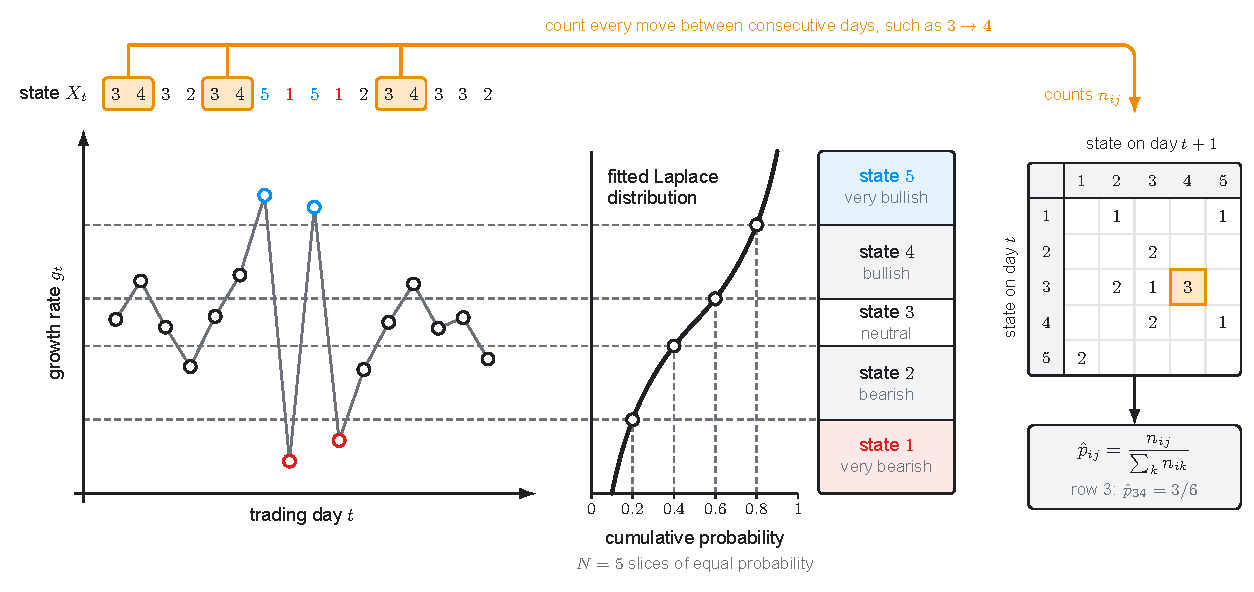
\includegraphics[width=\textwidth,height=0.66\textheight,keepaspectratio]{../figs/Fig-L13a-JumpHMM-Fit-Schematic.pdf}
  \end{center}
\end{frame}

\begin{frame}{Algorithm: Fit the Model}
  Given the daily growth rates $g_{1},\dotsc,g_{T}$ of one ticker, the number of states
  $N$, and $\nu$:
  \begin{enumerate}\setlength{\itemsep}{0.3em}
    \item \hilite{Laplace}: $\mu\gets$ the median of the growth rates, and
      $b\gets\frac{1}{T}\sum_{t}\lvert g_{t}-\mu\rvert$.
    \item \hilite{States}: $X_{t}\gets s_{k}$, where $(k-1)/N\leq F_{L}(g_{t})<k/N$.
    \item \hilite{Count}: $n_{ij}\gets n_{ij}+1$ for each move from $X_{t-1}=s_{i}$ to $X_{t}=s_{j}$.
    \item \hilite{Transitions}: $\hat{p}_{ij}\gets n_{ij}/\sum_{k}n_{ik}$.
    \item \hilite{Emissions}: $\mu_{k}$, $\sigma_{k}\gets$ the mean and standard deviation of
      the growth rates of the days in state $s_{k}$.
    \item \hilite{Start}: compute the stationary distribution $\bar{\pi}$ of $\hat{\Pb}$.
  \end{enumerate}
  \slidenote{Full version:}{the lecture notebook}
\end{frame}

\begin{frame}{Why Add Jumps?}
  The counted chain forgets quickly: after a volatile day, a few transitions usually
  return it to the middle states, so $|g_{t}|$ is correlated for only a few days.
  \hilite{Jump episodes} keep volatile periods going:
  \begin{itemize}\setlength{\itemsep}{0.35em}
    \item With no episode under way, an episode starts with probability $\epsilon$.
    \item It lasts a Poisson number of days with mean $\lambda$.
    \item Each episode day is drawn from the few most extreme states, negative or
      positive: a run of large moves of both signs.
  \end{itemize}
\end{frame}

\begin{frame}{The Jump Hidden Markov Model: One Day}
  An ordinary day steps with $\hat{\Pb}$. An episode day draws its state from the most
  negative or the most positive states:
  \begin{center}
    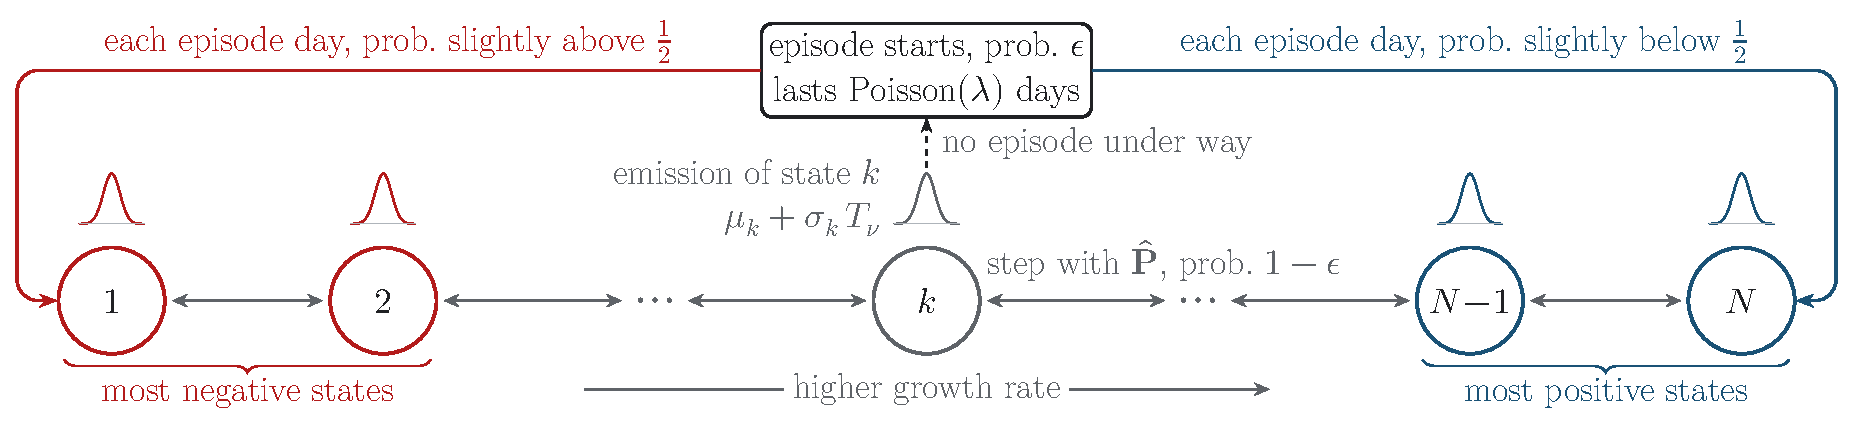
\includegraphics[width=\textwidth,height=0.58\textheight,keepaspectratio]{../figs/Fig-L13a-JumpHMM-Schematic.pdf}
  \end{center}
\end{frame}

\begin{frame}{Algorithm: Sample a Path}
  Draw $X_{1}\sim\bar{\pi}$ and $g_{1}$ from its emission, and set
  $\texttt{remaining}\gets 0$. Each day $t=2,\dotsc,T$ runs in this order:
  \begin{enumerate}\setlength{\itemsep}{0.3em}
    \item \hilite{New episode}: if $\texttt{remaining}=0$, draw $u\sim\text{Uniform}(0,1)$.
      If $u<\epsilon$, draw $\texttt{remaining}\sim\text{Poisson}(\lambda)$.
    \item \hilite{Episode day}: if $\texttt{remaining}>0$, draw $X_{t}$ uniformly from the
      most negative states $\Sc_{-}$ with probability $p_{\text{neg}}$, otherwise from the
      most positive states $\Sc_{+}$. Set $\texttt{remaining}\gets\texttt{remaining}-1$.
    \item \hilite{Ordinary day}: if $\texttt{remaining}=0$, draw $X_{t}$ from row
      $X_{t-1}$ of $\hat{\Pb}$.
    \item \hilite{Emission}: $g_{t}\gets\mu_{k}+\sigma_{k}\,T_{\nu}$, where $X_{t}=s_{k}$.
  \end{enumerate}
  \slidenote{Full version:}{the lecture notebook}
\end{frame}

\begin{frame}{Tuning and Checking the Model}
  A grid search picks $(\epsilon,\lambda)$. On the $M$ simulated paths with an episode,
  it scores each path's autocorrelation $\hat{\rho}_{m,k}$ of $|g_{t}|$ and kurtosis
  $\hat{\kappa}_{m}$ against the data's $\rho_{k}$, $\kappa$:
  \begin{equation*}
    J(\epsilon,\lambda)=\frac{1}{M}\sum_{m=1}^{M}\Bigl[\sum_{k=1}^{25}\left(\rho_{k}-\hat{\rho}_{m,k}\right)^{2}+0.2\left(\kappa-\hat{\kappa}_{m}\right)^{2}\Bigr]
  \end{equation*}
  The score is noisy, so the chosen pair can change with the seed.
  \slidenote{Example:}{\href{\repo/CHEME-5660-L13a-Example-JumpHMM-SPY-Fall-2026.ipynb}{\dimmed{CHEME-5660-L13a-Example-JumpHMM-SPY-Fall-2026.ipynb}}}
\end{frame}

% ========== Many Assets
\begin{frame}{Review: Factor Models}
  Previously, we studied \hilite{factor models}, which explain how stocks move together
  with a few common factors:
  \begin{equation*}
    g_{i}(t)=\underbrace{\alpha_{i}}_{\textstyle\text{firm}}+\underbrace{\beta_{i}\,g_{m}(t)}_{\textstyle\text{market}}+\underbrace{\textstyle\sum_{j}\delta_{ij}\,f_{j}(t)}_{\textstyle\text{other factors}}+\underbrace{\varepsilon_{i}(t)}_{\textstyle\text{residual}}
  \end{equation*}
  The \hilite{single index model} keeps only the market factor. It assumes that the
  residuals of different stocks are uncorrelated, which means that only the market links
  two stocks. In the data, the residuals of stocks in the same sector, such as two banks,
  are correlated.
\end{frame}

\begin{frame}{Many Assets: The Sector Factor Model}
  \textbf{\ink{Definition:}} in the \hilite{sector factor model}, each stock has one other
  factor besides the market, the factor $f_{s}$ of its sector $s$. The daily growth rate
  of stock $i$ in sector $s$ is given by:
  \begin{equation*}
    g_{i}(t)=\alpha_{i}+\beta_{i}\,\underbrace{g_{m}(t)}_{\textstyle\text{market}}+\delta_{i}\,\underbrace{f_{s}(t)}_{\textstyle\text{sector}}+\psi_{i}\,\underbrace{\tilde{\varepsilon}_{i}(t)}_{\textstyle\text{own}}
  \end{equation*}
  Here $\alpha_{i}$ and $\beta_{i}$ are the single index estimates, held fixed. The sector
  draw $f_{s}$ models the sector's average residual, with loading $\delta_{i}$. The own draw
  $\tilde{\varepsilon}_{i}$ models the stock, centered and scaled by $\psi_{i}$ so its
  variance matches the real one on average. Each draw is a jump hidden Markov model, and
  the shared draws are the only link between stocks.
\end{frame}

\begin{frame}{What the Model Keeps and Gives Up}
  Composing stocks from shared draws on the same day has consequences:
  \begin{itemize}\setlength{\itemsep}{0.45em}
    \item \hilite{Keeps}: fat tails and clustered volatility in every draw; stocks in a
      sector move together through their shared sector draw, all stocks through the
      market draw.
    \item \hilite{Gives up}: sector draws are independent, so stocks in different
      sectors are linked only through the market.
    \item \hilite{No copula}: a copula reorders each stock's draws across days and would
      scramble the timing of the volatile periods and jump episodes in them.
  \end{itemize}
\end{frame}

\begin{frame}{An Option: A Drifting $\beta$}
  Holding $\beta_{i}$ fixed is a simplification: real $\beta$ wanders. The model can let
  $\beta_{i}(t)$ drift around $\hat{\beta}_{i}$ as an exponential moving average of random
  shocks, sized by how much the online estimate of $\beta$ wanders in the real data.

  \vspace{0.5em}
  A trading method that re-estimates $\beta$ as it trades then faces the same problem
  in the synthetic market as in the real one.
  \slidenote{Example:}{\href{\repo/CHEME-5660-L13a-Example-JumpHMM-SectorFactor-Fall-2026.ipynb}{\dimmed{CHEME-5660-L13a-Example-JumpHMM-SectorFactor-Fall-2026.ipynb}}}
\end{frame}

% ========== Optional advanced material
\begin{frame}{Optional Advanced Material}
  \vspace{0.4em}
  {\normalsize\textbf{\ink{Markov models:}} \dimmed{advanced/markov/}\par
  \href{\repo/advanced/markov/CHEME-5660-L13a-Lecture-MarkovModels-Fall-2026.ipynb}{\dimmed{CHEME-5660-L13a-Lecture-MarkovModels-Fall-2026.ipynb}}}

  \vspace{0.6em}
  The Markov property, the stationary distribution by power iteration, and the sampling
  algorithm of a hidden Markov model. Two examples apply a hidden Markov model to a
  person's mood and to the daily growth rate of \texttt{SPY}.
\end{frame}

\begin{frame}{Summary}
  \vspace{0.3em}
  We built synthetic markets for stress tests, from Markov chains to a jump hidden
  Markov model of one asset and a sector factor model of many stocks.

  \vspace{0.4em}
  {\large\textbf{\ink{Key takeaways}}}
  \begin{itemize}\setlength{\itemsep}{0.4em}
    \item \hilite{Markov chains}: states, a transition matrix estimated by counting,
      and a stationary distribution; hidden states emit what we observe.
    \item \hilite{Jump hidden Markov model}: fat tails from binned Student-t states, and
      part of the volatility clustering from tuned jump episodes.
    \item \hilite{Sector factor model}: shared market and sector draws make synthetic
      stocks move together.
  \end{itemize}
  \vspace{0.3em}
  Synthetic markets let us test a method on many paths, not one.
\end{frame}

\end{document}
